\begin{appendices}
\section{All configurations for surface decoder in this paper}
\begin{table*}
	\caption{Configurations for surface decoders(1/3)}
	\label{tab:surf_dec1}
	\centering
	\begin{tabular}{| l | l | l | l }
		\hline
		\hline
		\#&surface decoders & \#trainable variable & training time \\
		\hline
		001&$CM^{1024,512,256}$ (aka. AtlasNet\cite{atlasnet})&~&~\\
		002&$CM^{1024,512}$ (baseline)&~&~\\
		003&$OM^{1024,512}$ &~&~\\
		004&$K^{4,512}M^{1024,512}$ &~&~\\
		005&$K^{8,512}M^{1024,512}$ &~&~\\
		006&$K^{16,512}M^{1024,512}$ &~&~\\
		007&$K^{4,1024}M^{1024,512}$ &~&~\\
		008&$K^{8,1024}M^{1024,512}$ &~&~\\
		009&$K^{16,1024}M^{1024,512}$ &~&~\\
		010&$K^{4,2048}M^{1024,512}$ &~&~\\
		011&$K^{8,2048}M^{1024,512}$ &~&~\\
		012&$K^{16,2048}M^{1024,512}$ &~&~\\
		013&$CP^4R^{4,64}$ &~&~\\
		014&$CP^{8}R^{8,64}$ &~&~\\
		015&$CP^{16}R^{16,64}$ &~&~\\
		016&$OP^4R^{4,64}$ &~&~\\
		017&$OP^{8}R^{8,64}$ &~&~\\
		018&$OP^{16}R^{16,64}$ &~&~\\
		019&$K^{4,512}P^{8}R^{8,64}$ &~&~\\
		020&$K^{8,512}P^{12}R^{12,64}$ &~&~\\
		021&$K^{16,512}P^{16}R^{16,64}$ &~&~\\
		022&$K^{4,1024}P^{4}R^{4,64}$ &~&~\\
		023&$K^{8,1024}P^{8}R^{8,64}$ &~&~\\
		024&$K^{16,1024}P^{16}R^{16,64}$ &~&~\\
		025&$K^{4,2048}P^{4}R^{4,64}$ &~&~\\
		026&$K^{8,2048}P^{8}R^{8,64}$ &~&~\\
		027&$K^{16,2048}P^{16}R^{16,64}$ &~&~\\
		\hline
		028&$(CM^{1024,512})_2$ (aka. FoldingNet\cite{foldingnet})&~&~\\
		029&$(OM^{1024,512})_2$ &~&~\\
		030&$(K^{4,512}M^{1024,512})_2$ &~&~\\
		031&$(K^{8,512}M^{1024,512})_2$ &~&~\\
		032&$(K^{16,512}M^{1024,512})_2$ &~&~\\
		033&$(K^{4,1024}M^{1024,512})_2$ &~&~\\
		034&$(K^{8,1024}M^{1024,512})_2$ &~&~\\
		035&$(K^{16,1024}M^{1024,512})_2$ &~&~\\
		036&$(K^{4,2048}M^{1024,512})_2$ &~&~\\
		037&$(K^{8,2048}M^{1024,512})_2$ &~&~\\
		038&$(K^{16,2048}M^{1024,512})_2$ &~&~\\
		039&$CP^4R^{4,64}_2$ &~&~\\
		040&$CP^{8}R^{8,64}_2$ &~&~\\
		041&$CP^{16}R^{16,64}_2$ &~&~\\
		042&$OP^4R^{4,64}_2$ &~&~\\
		043&$OP^{8}R^{8,64}_2$ &~&~\\
		044&$OP^{16}R^{16,64}_2$ &~&~\\
		045&$K^{4,512}P^{4}R^{4,64}_2$ &~&~\\
		046&$K^{8,512}P^{8}R^{8,64}_2$ &~&~\\
		047&$K^{16,512}P^{16}R^{16,64}_2$ &~&~\\
		048&$K^{4,1024}P^{4}R^{4,64}_2$ &~&~\\
		049&$K^{8,1024}P^{8}R^{8,64}_2$ &~&~\\
		050&$K^{16,1024}P^{16}R^{16,64}_2$ &~&~\\
		051&$K^{4,2048}P^{4}R^{4,64}_2$ &~&~\\
	\end{tabular}
\end{table*}
\begin{table*}
	\caption{Configurations for surface decoders(2/3)}
	\label{tab:surf_dec2}
	\centering
	\begin{tabular}{|l | l | l | l }
		\hline
		\hline
		\# & surface decoders & \#trainable variable & training time \\
		\hline
		052&$K^{8,2048}P^{8}R^{8,64}_2$ &~&~\\
		053&$K^{16,2048}P^{16}R^{16,64}_2$ &~&~\\
		054&$(CP^4R^{4,64})_2$ &~&~\\
		055&$(CP^{8}R^{8,64})_2$ &~&~\\
		056&$(CP^{16}R^{16,64})_2$ &~&~\\
		057&$(OP^4R^{4,64})_2$ &~&~\\
		058&$(OP^{8}R^{8,64})_2$ &~&~\\
		059&$(OP^{16}R^{16,64})_2$ &~&~\\
		060&$(K^{4,512}P^{4}R^{4,64})_2$ &~&~\\
		061&$(K^{8,512}P^{8}R^{8,64})_2$ &~&~\\
		062&$(K^{16,512}P^{16}R^{16,64})_2$ &~&~\\
		063&$(K^{4,1024}P^{4}R^{4,64})_2$ &~&~\\
		064&$(K^{8,1024}P^{8}R^{8,64})_2$ &~&~\\
		065&$(K^{16,1024}P^{16}R^{16,64})_2$ &~&~\\
		066&$(K^{4,2048}P^{4}R^{4,64})_2$ &~&~\\
		067&$(K^{8,2048}P^{8}R^{8,64})_2$ &~&~\\
		068&$(K^{16,2048}P^{16}R^{16,64})_2$ &~&~\\
		\hline
		069&$(CM^{1024,512})_4$ &~&~\\
		070&$(OM^{1024,512})_4$ &~&~\\
		071&$(K^{8,512}M^{1024,512})_4$ &~&~\\
		072&$(K^{12,512}M^{1024,512})_4$ &~&~\\
		073&$(K^{16,512}M^{1024,512})_4$ &~&~\\
		074&$(K^{8,1024}M^{1024,512})_4$ &~&~\\
		075&$(K^{12,1024}M^{1024,512})_4$ &~&~\\
		076&$(K^{16,1024}M^{1024,512})_4$ &~&~\\
		077&$(K^{8,2048}M^{1024,512})_4$ &~&~\\
		078&$(K^{12,2048}M^{1024,512})_4$ &~&~\\
		079&$(K^{16,2048}M^{1024,512})_4$ &~&~\\
		080&$CP^8R^{8,64}_4$ &~&~\\
		081&$CP^{12}R^{12,64}_4$ &~&~\\
		082&$CP^{16}R^{16,64}_4$ &~&~\\
		083&$OP^8R^{8,64}_4$ &~&~\\
		084&$OP^{12}R^{12,64}_4$ &~&~\\
		085&$OP^{16}R^{16,64}_4$ &~&~\\
		086&$K^{8,512}P^{8}R^{8,64}_4$ &~&~\\
		087&$K^{12,512}P^{12}R^{12,64}_4$ &~&~\\
		088&$K^{16,512}P^{16}R^{16,64}_4$ &~&~\\
		089&$K^{8,1024}P^{8}R^{8,64}_4$ &~&~\\
		090&$K^{12,1024}P^{12}R^{12,64}_4$ &~&~\\
		091&$K^{16,1024}P^{16}R^{16,64}_4$ &~&~\\
		092&$K^{8,2048}P^{8}R^{8,64}_4$ &~&~\\
		093&$K^{12,2048}P^{12}R^{12,64}_4$ &~&~\\
		094&$K^{16,2048}P^{16}R^{16,64}_4$ &~&~\\
		095&$(CP^8R^{8,64})_4$ &~&~\\
		096&$(CP^{12}R^{12,64})_4$ &~&~\\
		097&$(CP^{16}R^{16,64})_4$ &~&~\\
		098&$(OP^8R^{8,64})_4$ &~&~\\
		099&$(OP^{12}R^{12,64})_4$ &~&~\\
		100&$(OP^{16}R^{16,64})_4$ &~&~\\
	\end{tabular}
\end{table*}
\begin{table*}
	\caption{Configurations for surface decoders(3/3)}
	\label{tab:surf_dec3}
	\centering
	\begin{tabular}{| l | l | l | l}
		\hline
		\hline
		\#&surface decoders & \#trainable variable & training time \\
		\hline
		101&$(K^{8,512}P^{8}R^{8,64})_4$ &~&~\\
		102&$(K^{12,512}P^{12}R^{12,64})_4$ &~&~\\
		103&$(K^{16,512}P^{16}R^{16,64})_4$ &~&~\\
		104&$(K^{8,1024}P^{8}R^{8,64})_4$ &~&~\\
		105&$(K^{12,1024}P^{12}R^{12,64})_4$ &~&~\\
		106&$(K^{16,1024}P^{16}R^{16,64})_4$ &~&~\\
		107&$(K^{8,2048}P^{8}R^{8,64})_4$ &~&~\\
		108&$(K^{12,2048}P^{12}R^{12,64})_4$ &~&~\\
		109&$(K^{16,2048}P^{16}R^{16,64})_4$ &~&~\\
		\hline
		110&$(CM^{1024,512})_2L$ &~&~\\
		111&$(CM^{1024,512}L)_2$ &~&~\\
		112&$(OM^{1024,512})_2L$ &~&~\\
		113&$(OM^{1024,512}L)_2$ &~&~\\
		114&$(K^{16,2048}M^{1024,512}L)_2$ &~&~\\
		115&$(K^{16,2048}M^{1024,512})_2L$ &~&~\\
		116&$CP^{16}R^{16,64}_2L$ &~&~\\
		117&$CP^{16}(R^{16,64}L)_2$ &~&~\\
		118&$OP^{16}R^{16,64}_2L$ &~&~\\
		119&$OP^{16}(R^{16,64}L)_2$ &~&~\\
		120&$K^{16,2048}P^{8}R^{8,64}_2L$ &~&~\\
		121&$K^{16,2048}P^{8}(R^{8,64}L)_2$ &~&~\\
	\end{tabular}
\end{table*}
\newpage
\section{Experiment on Laplacian}
\begin{table*}
\label{tab:lpl}
\centering
\begin{tabular}{| l | l |}
model  &   0 epoch   \\
\hline
origin &   0.0051685 \\
cot    &   0.0051651 \\
2 cot   &  0.0051598 \\
graph   &  0.0051679 \\
2 graph &  0.0051687 \\
\end{tabular}
\end{table*}
\begin{figure}[htbp]
	\centering
%	\includegraphics[width=\linewidth]{img/appendix/atlasnetvsour.png}
	\caption{Add Laplace to AtlasNet}
	\label{fig:atlasnet_lpl}
\end{figure}
\newpage
\section{More Results}
\begin{figure*}[htbp]
	\centering
	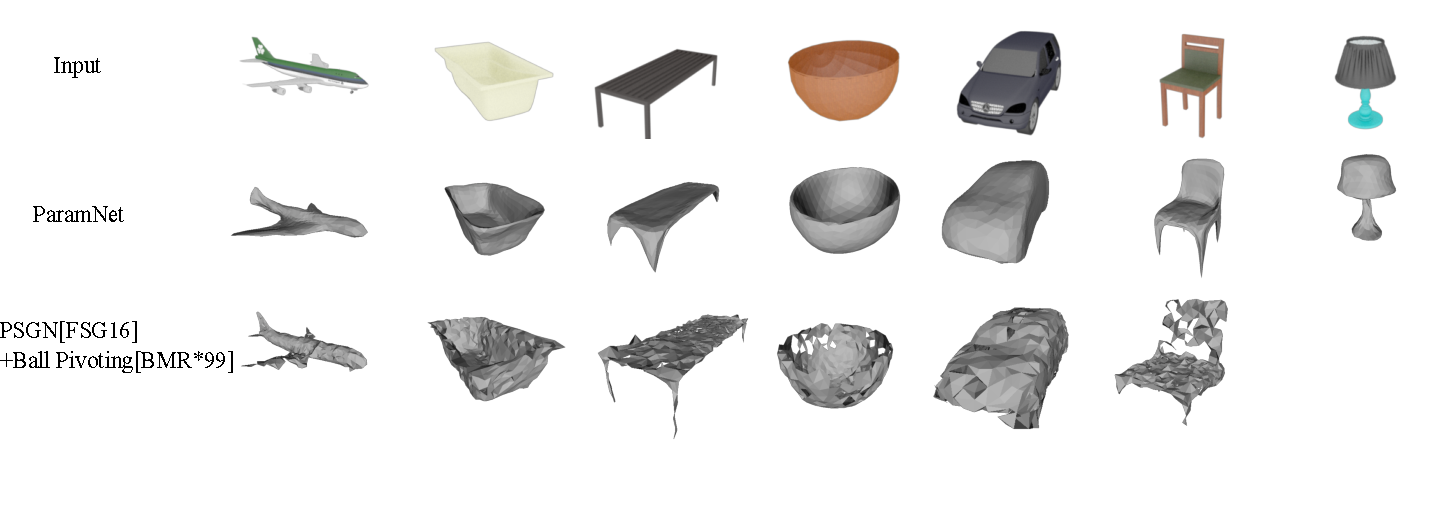
\includegraphics[width=\linewidth]{img/more_res/res}
	\caption{More visual results randomly picked from testing data}
	\label{fig:more_res}
\end{figure*}
\begin{table*}
	\label{tab:pix2mesh}
	\centering
	\begin{tabular}{| l | l |}
		model  &   0 epoch   \\
		\hline
		Pix2Mesh &   0.59 \\
		Pix2Mesh with KnPointNet instead of graph conv &   0.63 \\
	\end{tabular}
\end{table*}
\begin{table*}
	\label{tab:concate}
	\centering
	\begin{tabular}{| l | l |}
		model  &   0 epoch   \\
		\hline
		Pix2Mesh &   0.59 \\
		Pix2Mesh with Laplace &   0.601 \\
	\end{tabular}
\end{table*}
\end{appendices}